%%%%%%%%%%%%%%%%%%%%%%%%%%%%%%%%%%%%%%%%%
% University/School Laboratory Report
% LaTeX Template
% Version 3.1 (25/3/14)
%
% This template has been downloaded from:
% http://www.LaTeXTemplates.com
%
% Original author:
% Linux and Unix Users Group at Virginia Tech Wiki 
% (https://vtluug.org/wiki/Example_LaTeX_chem_lab_report)
%
% License:
% CC BY-NC-SA 3.0 (http://creativecommons.org/licenses/by-nc-sa/3.0/)
%
%%%%%%%%%%%%%%%%%%%%%%%%%%%%%%%%%%%%%%%%%

%----------------------------------------------------------------------------------------
%	PACKAGES AND DOCUMENT CONFIGURATIONS
%----------------------------------------------------------------------------------------

\documentclass{article}

\usepackage[version=3]{mhchem} % Package for chemical equation typesetting
\usepackage{siunitx} % Provides the \SI{}{} and \si{} command for typesetting SI units
\usepackage{graphicx} % Required for the inclusion of images
\usepackage{natbib} % Required to change bibliography style to APA
\usepackage{amsmath} % Required for some math elements 
\usepackage{hyperref}
\usepackage{fontspec}
\usepackage{caption}
\usepackage{subcaption}
\usepackage{xcolor}

\usepackage[left=2cm, right=2cm, top=2cm]{geometry}
\definecolor{dark-blue}{rgb}{0.15,0.15,0.4}
\hypersetup{colorlinks,linkcolor={dark-blue},citecolor={dark-blue},urlcolor={dark-blue}}

% the main font, with all features on
\setmainfont
[ ExternalLocation ,
      Mapping          = tex-text ,
      Numbers          = OldStyle ,
      Ligatures        = {Common,Contextual} ,
      BoldFont         = texgyrepagella-bold.otf ,
      ItalicFont       = texgyrepagella-italic.otf ,
      BoldItalicFont   = texgyrepagella-bolditalic.otf ]
      {texgyrepagella-regular.otf}
    
  % same like the main font, but without old-style nums
  \newfontfamily\newnums
    [ ExternalLocation ,
      Mapping          = tex-text ,
      Ligatures        = {Common,Contextual} ,
      BoldFont         = texgyrepagella-bold.otf ,
      ItalicFont       = texgyrepagella-italic.otf ,
      BoldItalicFont   = texgyrepagella-bolditalic.otf ]
    {texgyrepagella-regular.otf}

\setlength\parindent{0pt} % Removes all indentation from paragraphs

\renewcommand{\labelenumi}{\alph{enumi}.} % Make numbering in the enumerate environment by letter rather than number (e.g. section 6)

\newcommand{\hmwkAuthorName}{
  Rihan \textsc{Stephen Pereira} \\
  \texttt{rihanstephen.pereira576@myci.csuci.edu, studentID - 002497665}
  \and
  Niranjan \textsc{Pawar}\\
  \texttt{niranjan.pawar987@myci.csuci.edu, studentID - 002718379}
}
%\usepackage{times} % Uncomment to use the Times New Roman font

%----------------------------------------------------------------------------------------
%	DOCUMENT INFORMATION
%----------------------------------------------------------------------------------------

\title{COMP 590 - Android Development \\ SEDaily - P3 Design} % Title

\author{\hmwkAuthorName} % Author name

\date{\today} % Date for the report

\begin{document}

\maketitle % Insert the title, author and date

\begin{center}
\begin{tabular}{l r}
Instructor: & Prof. Brian Thoms% Instructor/supervisor
\end{tabular}
\end{center}


%----------------------------------------------------------------------------------------
%	SECTION 1
%----------------------------------------------------------------------------------------
The Software Engineering Daily(SEDaily) is a open source project welcoming developers to hack on
its existing repositories and also propose new projects that add value to its users. Its ecosystem
comprises of - 

\begin{itemize}
\item Backend services
  \begin{itemize}
    \item REST API - serves as a backend for android/ios/frontend(vue.js)
    \item Miner - source of all data for SE daily ecosystem
    \item logging and analytics
  \end{itemize} 
\item Vue.js(frontend)
\item Android app
\item IOS app
\end{itemize}

\clearpage

\section{Architecture/System Diagrams}
\begin{figure}[h]
  \centering
  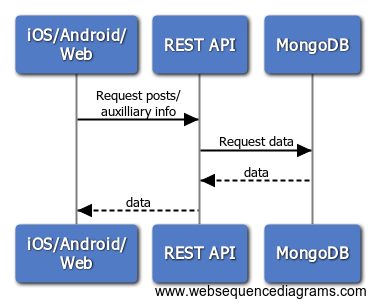
\includegraphics[width=.5\linewidth]{img/system_diagram.png}
  \caption{sedaily system diagram, source - \href{https://www.softwaredaily.com/}{softwaredaily.com}}
\end{figure}

\begin{figure}[h]
  \centering
  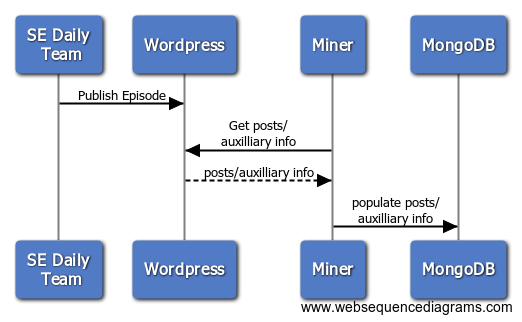
\includegraphics[width=.7\linewidth]{img/data_miner.png}
  \caption{The data miner pulls episodes from wordpress and saves to mongoDB, source - \href{https://www.softwaredaily.com/}{softwaredaily.com}}
\end{figure}
\pagebreak

%----------------------------------------------------------------------------------------
%	SECTION 2
%----------------------------------------------------------------------------------------
\section{Use Case Diagrams}
\begin{figure}[h]
  \centering
  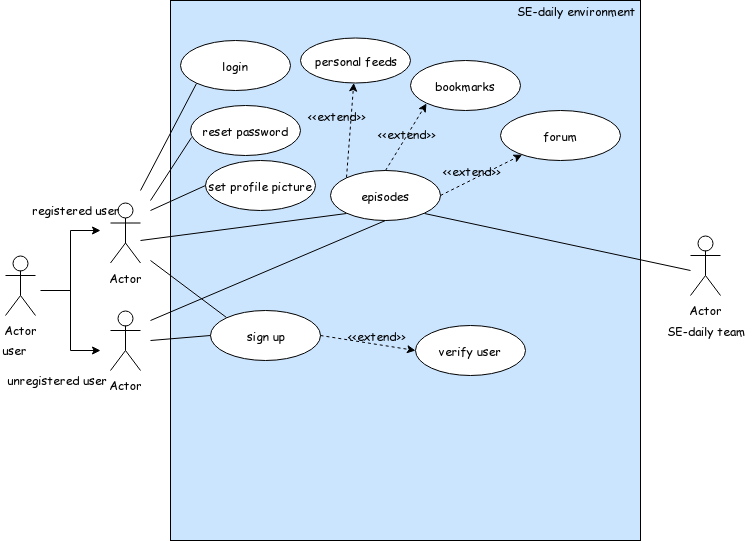
\includegraphics[width=.9\linewidth]{img/use_case.png}
  \caption{Use-case diagram showing interaction between user and SEdaily software components}
\end{figure}

\pagebreak

%----------------------------------------------------------------------------------------
%	SECTION 3
%----------------------------------------------------------------------------------------
\section{App Interface Mockups}
\begin{figure}[h]
\centering
\begin{minipage}{.5\textwidth}
  \centering
  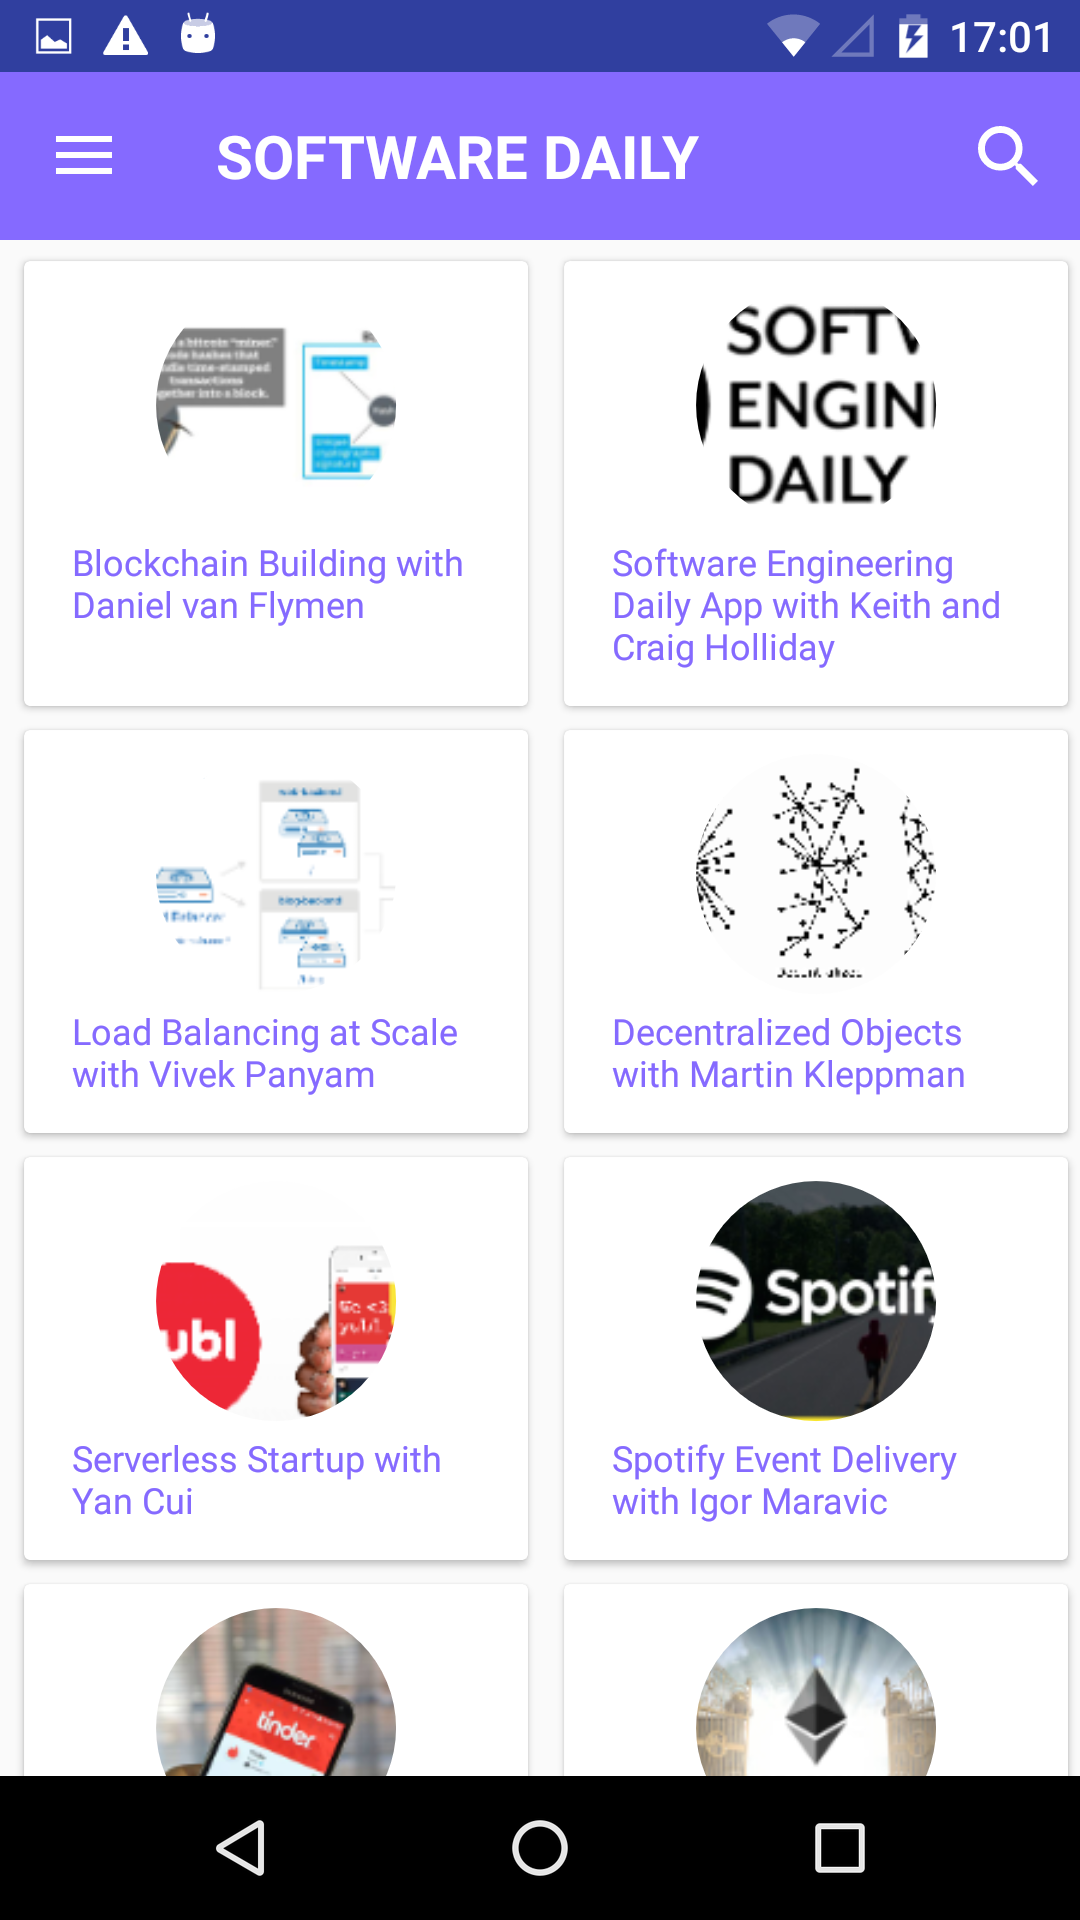
\includegraphics[width=.4\linewidth]{img/sedaily_main.png}
  \captionof{figure}{grid view \& default main activity}
\end{minipage}%
\begin{minipage}{.7\textwidth}
  \centering
  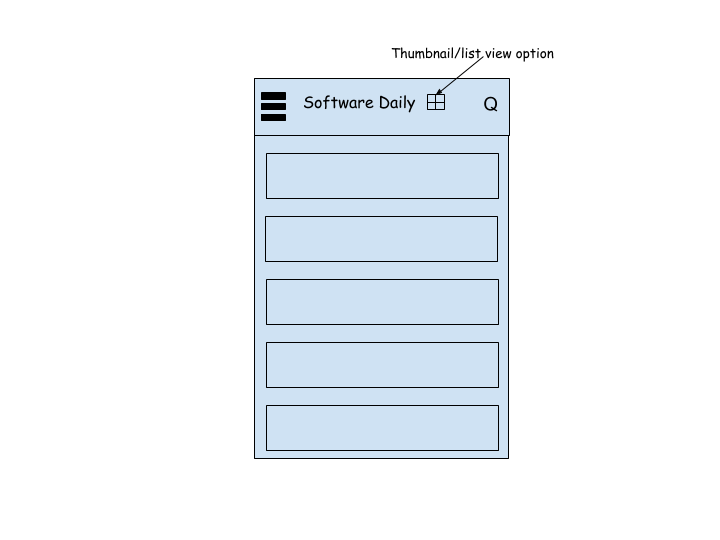
\includegraphics[width=.9\linewidth]{img/list_view.png}
  \captionof{figure}{list view with list/grid toggle button}
\end{minipage}
\end{figure}

\begin{figure}[h]
\centering
\begin{minipage}{.6\textwidth}
  \centering
  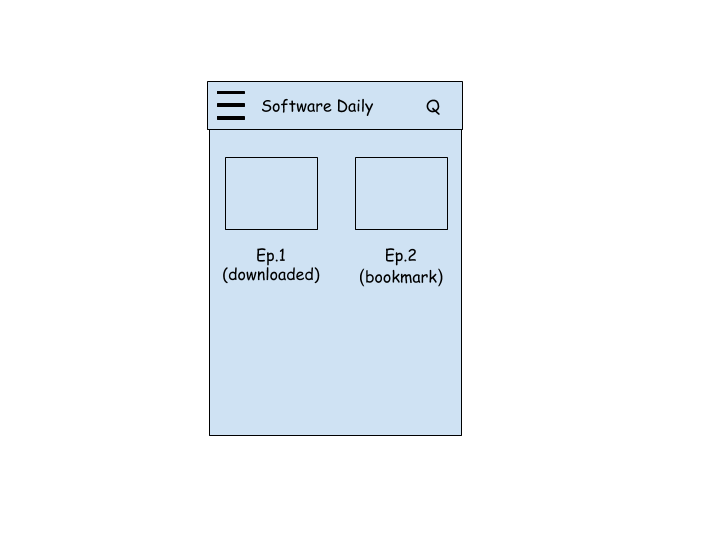
\includegraphics[width=10cm,height=8cm]{img/bookmarks.png}
  \captionof{figure}{downloaded and bookmark episodes view mockup}
\end{minipage}%
\begin{minipage}{.5\textwidth}
  \centering
  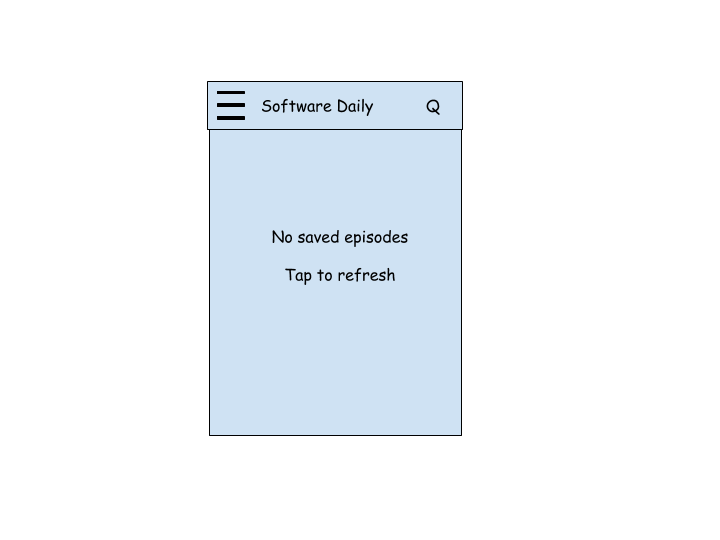
\includegraphics[width=10cm,height=8cm]{img/bookmarks_mockup.png}
  \captionof{figure}{empty bookmark view mockup}
\end{minipage}
\end{figure}

\begin{figure}[h]
\centering
\begin{minipage}{.5\textwidth}
  \centering
  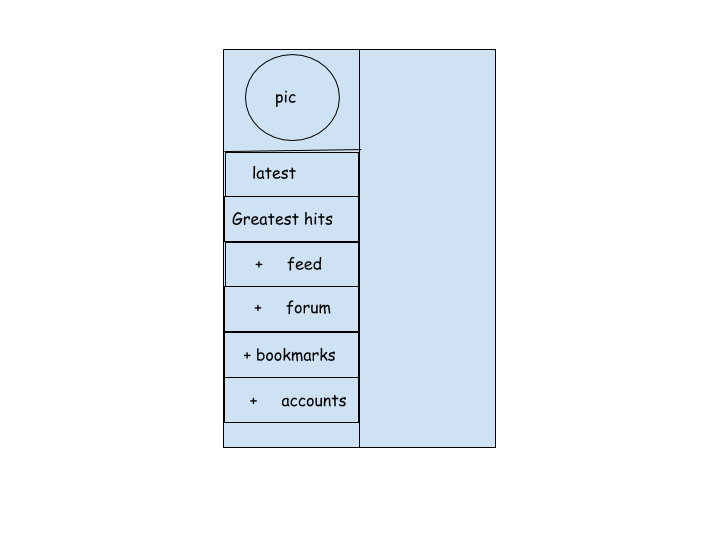
\includegraphics[width=10cm, height=8cm]{img/side_menu.png}
  \captionof{figure}{side-menu bar, \+ will be the new additions}
\end{minipage}%
\begin{minipage}{.7\textwidth}
  \centering
  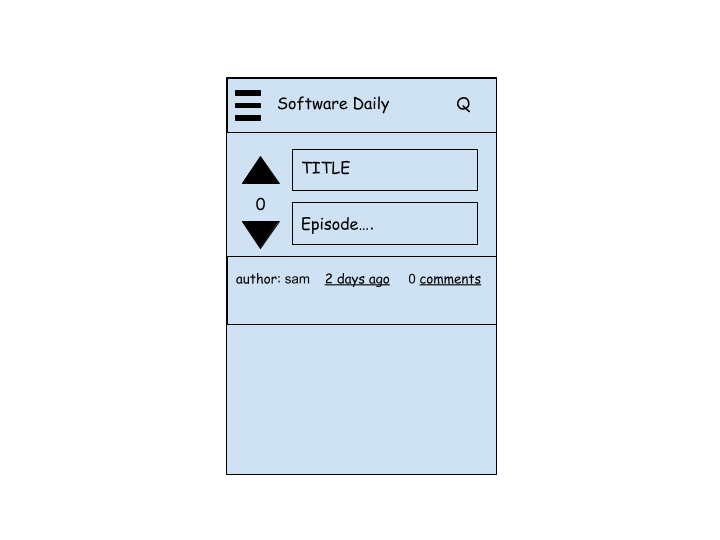
\includegraphics[width=.9\linewidth]{img/forum.png}
  \captionof{figure}{Forum integration mockup}
\end{minipage}
\end{figure}

\end{document}
%%% Local Variables:
%%% mode: latex
%%% TeX-master: t
%%% End:
